\documentclass[14pt]{extarticle} %Класс позволяет использовать базовые шрифты бОльших размеров
\usepackage{imit_vkr}

%=============================
%Персональная настройка макета
%Здесь могут располагаться дополнительные команды для персональной тонкой настройки
%=============================

%=============================
%Конец Персональная настройка макета
%=============================

%Подключение литературы
\addbibresource{literature.bib}


\begin{document}
	
%%%--------Титульная страница
%==Титульная страница
\thispagestyle{empty}
\begin{center}
Министерство науки и высшего образования Российской Федерации\\
Федеральное государственное бюджетное образовательное\\
учреждение высшего образования\\
<<Иркутский государственный университет>>\\
(ФГБОУ ВО <<ИГУ>>)\\
Институт математики и информационных технологий\\
Кафедра алгебраических и информационных систем\\
\end{center}

\vspace{2.7cm}

\begin{center}
{\bf 
ВЫПУСКНАЯ КВАЛИФИКАЦИОННАЯ РАБОТА
БАКАЛАВРА\\[1mm]
по направлению <<09.03.03 Прикладная информатика>>\\[1mm]
профиль подготовки <<Информационная сфера>>
}  

\vspace{0.9cm}

{
ПОСТРОЕНИЕ УНИВЕРСАЛЬНОЙ 
ТЕСТОВОЙ СИСТЕМЫ\\[1mm]
ДЛЯ ИНФОРМАЦИОННО-ОБРАЗОВАТЕЛЬНОЙ СРЕДЫ 
} %Текст должен быть набран ЗАГЛАВНЫМИ БУКВАМИ
\end{center}

\vspace{1.8cm}

{
\noindent\hbox to 0.48\textwidth {%
	\mbox{ } \hfil} %
	\begin{tabular}[t]{l}
		Студент 4 курса очного отделения\\
		Группа 02461--ДБ\\
		Криштофенко Александр 
		Вячеславович		
	\end{tabular}		
}

\vspace{0.8cm}

{
\noindent\hbox to 0.48\textwidth {%	
	\mbox{ } \hfil} %
	\begin{tabular}[t]{l}
		Руководитель:\\ к.ф.-м.н., доцент\\
		\rule{2.7cm}{0.5pt} Казимиров А.С.		
	\end{tabular}		
}

\vspace{0.8cm}

{
	\noindent\hbox to 0.48\textwidth {%	
		\mbox{ } \hfil} %
	\begin{tabular}[t]{l}
		Допущена к защите\\
		Зав. кафедрой АиИС, д.ф.-м.н., доцент \\
		\rule{2.7cm}{0.5pt} Пантелеев В.И.
		%		\hfill <<\rule{1.0cm}{0.5pt}>> \rule{3.0cm}{0.5pt} 2016~г.		
	\end{tabular}		
}

\vspace{0.8cm}

\vfill 
\noindent
\begin{minipage}{\textwidth}
\centering	 Иркутск 2023
\end{minipage}
\newpage
%==Титульная страница
\thispagestyle{empty}
\begin{center}
Министерство науки и высшего образования Российской Федерации\\
Федеральное государственное бюджетное образовательное\\
учреждение высшего образования\\
<<Иркутский государственный университет>>\\
(ФГБОУ ВО <<ИГУ>>)\\
Институт математики и информационных технологий\\
Кафедра алгебраических и информационных систем\\
\end{center}

\vspace{1.7cm}

\begin{center}
{\bf 
ВЫПУСКНАЯ КВАЛИФИКАЦИОННАЯ РАБОТА
БАКАЛАВРА\\[1mm]
по направлению <<09.03.03 Прикладная информатика>>\\[1mm]
профиль подготовки <<Проектирование и разработка информационных систем>>
}  

\vspace{0.9cm}

{
ПОСТРОЕНИЕ УНИВЕРСАЛЬНОЙ 
ТЕСТОВОЙ СИСТЕМЫ\\[1mm]
ДЛЯ ИНФОРМАЦИОННО-ОБРАЗОВАТЕЛЬНОЙ СРЕДЫ 
} %Текст должен быть набран ЗАГЛАВНЫМИ БУКВАМИ
\end{center}

\vspace{1.3cm}

{
\noindent\hbox to 0.48\textwidth {%
	\mbox{ } \hfil} %
	\begin{tabular}[t]{l}
		Студент 4 курса очного отделения\\
		Группа 02461--ДБ\\
		Криштофенко Александр 
		Вячеславович		
	\end{tabular}		
}

\vspace{0.5cm}

{
	\noindent\hbox to 0.48\textwidth {%	
		\mbox{ } \hfil} %
	\begin{tabular}[t]{l}
		Руководитель:\\ к.ф.-м.н., доцент\\
		\rule{2.7cm}{0.5pt} Казимиров А.С.		
	\end{tabular}		
}

\vspace{0.5cm}

{
\noindent\hbox to 0.48\textwidth {%	
	\mbox{ } \hfil} %
	\begin{tabular}[t]{l}
		Консультант:\\
		генеральный директор \\
		ООО <<Информатика в образовании>>\\
		Реймеров С.Ю.		
	\end{tabular}		
}

\vspace{0.5cm}

{
	\noindent\hbox to 0.48\textwidth {%	
		\mbox{ } \hfil} %
	\begin{tabular}[t]{l}
		Допущена к защите\\
		Зав. кафедрой АиИС, д.ф.-м.н., доцент \\
		\rule{2.7cm}{0.5pt} Пантелеев В.И.
		%		\hfill <<\rule{1.0cm}{0.5pt}>> \rule{3.0cm}{0.5pt} 2016~г.		
	\end{tabular}		
}

\vspace{0.5cm}

\vfill 
\noindent
\begin{minipage}{\textwidth}
\centering	 Иркутск 2025
\end{minipage}
\newpage
%==Титульная страница
\thispagestyle{empty}
\begin{center}
Министерство науки и высшего образования Российской Федерации\\
Федеральное государственное бюджетное образовательное\\
учреждение высшего образования\\
<<Иркутский государственный университет>>\\
(ФГБОУ ВО <<ИГУ>>)\\
Институт математики и информационных технологий\\
Кафедра алгебраических и информационных систем\\
\end{center}

\vspace{2.7cm}

\begin{center}
{\bf 
ВЫПУСКНАЯ КВАЛИФИКАЦИОННАЯ РАБОТА
БАКАЛАВРА\\[1mm]
по направлению <<02.03.02 Фундаментальная информатика и \\[1mm]
информационные технологии>>\\[1mm]
профиль подготовки <<Фундаментальная информатика и \\[1mm] информационные технологии>>
}  

\vspace{0.9cm}

{
ПОСТРОЕНИЕ УНИВЕРСАЛЬНОЙ 
ТЕСТОВОЙ СИСТЕМЫ\\[1mm]
ДЛЯ ИНФОРМАЦИОННО-ОБРАЗОВАТЕЛЬНОЙ СРЕДЫ 
} %Текст должен быть набран ЗАГЛАВНЫМИ БУКВАМИ
\end{center}

\vspace{1.8cm}

{
\noindent\hbox to 0.48\textwidth {%
	\mbox{ } \hfil} %
	\begin{tabular}[t]{l}
		Студент 4 курса очного отделения\\
		Группа 02461--ДБ\\
		Криштофенко Александр 
		Вячеславович		
	\end{tabular}		
}

\vspace{0.8cm}

{
\noindent\hbox to 0.48\textwidth {%	
	\mbox{ } \hfil} %
	\begin{tabular}[t]{l}
		Руководитель:\\ к.ф.-м.н., доцент\\
		\rule{2.7cm}{0.5pt} Казимиров А.С.		
	\end{tabular}		
}

\vspace{0.8cm}

{
	\noindent\hbox to 0.48\textwidth {%	
		\mbox{ } \hfil} %
	\begin{tabular}[t]{l}
		Допущена к защите\\
		Зав. кафедрой АиИС, д.ф.-м.н., доцент \\
		\rule{2.7cm}{0.5pt} Пантелеев В.И.
		%		\hfill <<\rule{1.0cm}{0.5pt}>> \rule{3.0cm}{0.5pt} 2016~г.		
	\end{tabular}		
}

\vspace{0.8cm}

\vfill 
\noindent
\begin{minipage}{\textwidth}
\centering	 Иркутск 2025
\end{minipage}
\newpage
%==Титульная страница
\thispagestyle{empty}
\begin{center}
	Министерство науки и высшего образования Российской Федерации\\
	Федеральное государственное бюджетное образовательное\\
	учреждение высшего образования\\
	<<Иркутский государственный университет>>\\
	(ФГБОУ ВО <<ИГУ>>)\\
	Институт математики и информационных технологий\\
	Кафедра алгебраических и информационных систем\\
\end{center}

\vspace{2.7cm}

\begin{center}
	{\bf 
		ВЫПУСКНАЯ КВАЛИФИКАЦИОННАЯ РАБОТА
		БАКАЛАВРА\\[1mm]
		по направлению <<02.03.03 Математическое обеспечение и  \\[1mm] 
		администрирование информационных систем>>\\[1mm]
		профиль подготовки <<Общий>>
	}  
	
	\vspace{0.9cm}
	
	{
		ПОСТРОЕНИЕ УНИВЕРСАЛЬНОЙ 
		ТЕСТОВОЙ СИСТЕМЫ\\[1mm]
		ДЛЯ ИНФОРМАЦИОННО-ОБРАЗОВАТЕЛЬНОЙ СРЕДЫ 
	} %Текст должен быть набран ЗАГЛАВНЫМИ БУКВАМИ
\end{center}

\vspace{1.1cm}

{
	\noindent\hbox to 0.48\textwidth {%
		\mbox{ } \hfil} %
	\begin{tabular}[t]{l}
		Студент 4 курса очного отделения\\
		Группа 02461--ДБ\\
		Криштофенко Александр
		Вячеславович		
	\end{tabular}		
}

\vspace{0.8cm}

{
	\noindent\hbox to 0.48\textwidth {%	
		\mbox{ } \hfil} %
	\begin{tabular}[t]{l}
		Руководитель:\\ к.ф.-м.н., доцент\\
		\rule{2.7cm}{0.5pt} Казимиров А.С.		
	\end{tabular}		
}

\vspace{0.8cm}

{
	\noindent\hbox to 0.48\textwidth {%	
		\mbox{ } \hfil} %
	\begin{tabular}[t]{l}
		Допущена к защите\\
		Зав. кафедрой, д.ф.-м.н., доцент \\
		\rule{2.7cm}{0.5pt} Пантелеев В.И.
		%		\hfill <<\rule{1.0cm}{0.5pt}>> \rule{3.0cm}{0.5pt} 2016~г.		
	\end{tabular}		
}

\vspace{0.8cm}

\vfill 
\noindent
\begin{minipage}{\textwidth}
	\centering	Иркутск 2023
\end{minipage}
\newpage
%%%----------------------Содержание дипломной работы%%%
\renewcommand{\baselinestretch}{1.5}
\normalsize
%-------------
%Содержание
%-------------
\renewcommand{\contentsname}{СОДЕРЖАНИЕ}
\noindent\tableofcontents

%-------------
%Основная часть
%-------------
\mynonumbersection{ВВЕДЕНИЕ}

Итоговая государственная аттестация является обязательной для всех выпускников~\cite{jech:lst,Ros,lacan:s20f}.
Она призвана установить и адекватно оценить уровень подготовки будущих 
специалистов.

Итоговая государственная аттестация осуществляется государственными аттестационными 
комиссиями, основными функциями которых являются комплексная оценка уровня 
подготовки выпускника, решение вопроса о присвоении квалификации и выдача 
выпускнику соответствующего диплома о высшем образовании.

Форма и условия проведения аттестационных испытаний определяется профилирующей кафедрой.

Итоговая государственная аттестация выпускника университета включает в себя
защиту выпускной квалификационной работы в форме дипломной работы или проекта.

\setlength{\itemsep}{0mm}
Выпускная квалификационная работа (ВКР) информатика 
представляет собой законченную разработку (дипломный проект) в профессиональной области, 
в которой: 

%-----------локальное переопределение маркера списка
%Требуется для вывода номера в формате 1) 2) при использовании пунктов списка, начинающихся с 
%строчной буквы
\begin{enumerate}[label=\arabic*)]  
\item сформулирована актуальность и место решаемой задачи 
информационного обеспечения в предметной области;
\item анализируется литература и информация, полученная с помощью 
глобальных сетей, по функционированию подобных систем в данной области 
или в смежных предметных областях; 
\item определяются и конкретно описываются выбранные выпускником объемы, 
методы и средства решаемой задачи.
\end{enumerate}


Темы выпускных квалификационных работ определяются профилирующей кафедрой. 
Студенту предоставляется право выбора темы выпускной квалификационной работы 
вплоть до предложения своей тематики с обоснованием целесообразности ее разработки.

При подготовке выпускником квалификационной работы каждому студенту назначается 
руководитель, как правило, из числа преподавателей профилирующей кафедры.

Темы выпускных квалификационных работ и состав руководителей утверждаются приказом 
по университету. Выпускные квалификационные работы подлежат обязательному 
рецензированию. 

К защите выпускной квалификационной работы допускаются лица, завершившие полный курс 
обучения и успешно прошедшие все предшествующие аттестационные испытания, 
предусмотренные учебным планом. Студент, не прошедший в течение установленного 
срока всех испытаний, входящих в состав итоговой государственной аттестации, 
отчисляется из университета и получает академическую справку.



%=======================

\mysection{Название первой главы}
\mysubsection{Название первого параграфа}
Форма и условия проведения аттестационных испытаний определяется профилирующей кафедрой.

Итоговая государственная аттестация выпускника университета включает в себя
защиту выпускной квалификационной работы в форме дипломной работы или проекта.

Выпускная квалификационная работа (ВКР) информатика 
представляет собой законченную разработку (дипломный проект) в профессиональной области, 
в которой: 
\begin{enumerate}[label=\arabic*)]
\item сформулирована актуальность и место решаемой задачи 
информационного обеспечения в предметной области;
\item анализируется литература и информация, полученная с помощью 
глобальных сетей, по функционированию подобных систем в данной области 
или в смежных предметных областях; 
\item определяются и конкретно описываются выбранные выпускником объемы, 
методы и средства решаемой задачи.
\end{enumerate}

Стартовая страница веб-приложения представлена на рис.~\ref{first} первый раз встретился в дипломе.
\begin{figure}[h]
\centering
%Рамка только для изображений с белым фоном
\fbox{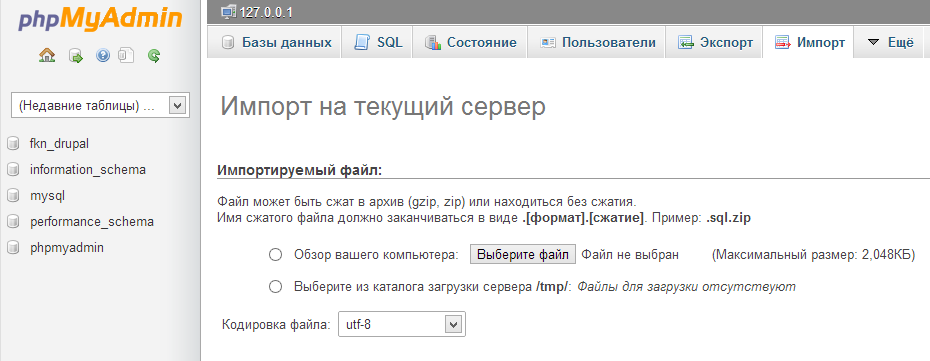
\includegraphics[scale=0.7]{img/import.png}}
\caption{Веб-приложение phpMyAdmin}
\label{first}
\end{figure}

\mysubsection{Название второго параграфа}

Все помещенные в ВКР иллюстрации (различные схемы, графики, фотографии) именуются рисунками. Размер рисунка не должен превышать принятого для ВКР формата бумаги. Подпись к рисунку размещается непосредственно под ним, выравнивание <<по ширине>>, со стандартным отступом слева. Рисунок помещается сразу после упоминания о нем в тексте. Каждая таблица должна иметь заголовок. Наименование <<Таблица>> с соответствующим номером, помещают над таблицей, используя выравнивание <<по правому краю>>, затем помещают заголовок, используя форматирование <<по центру>>. Сокращения слов в таблице недопустимы. Для всех приведенных в таблице характеристик должны быть указаны единицы измерения и их размерность. Если таблица располагается на нескольких страницах, то каждая последующая страница оформляется определенным образом. Над переносимой частью таблицы, справа пишется <<Продолжение табл.>> или <<Окончание табл.>> и указывается ее номер. При переносе части таблицы на другие страницы название помещают только над первой частью таблицы.

Таблицы и рисунки помещаются в тексте после абзацев, содержащих ссылку на них, а если такой возможности нет, то с первого абзаца на следующей странице. Нумерация таблиц и рисунков сквозная для всей ВКР.

Уравнения и формулы выделяются из текста в отдельную строку. Формула в отдельной строке должна располагаться по центру. Символьные составляющие и числовые коэффициенты формулы расшифровываются. Пояснения значений символов и числовых коэффициентов следует приводить непосредственно под формулой в той же последовательности, в которой они даны в формуле. Первую строку пояснения начинают со слова <<где>> без двоеточия. В конце каждой строки ставят точку с запятой, в конце последней --- точку. В тексте ссылки на формулу даются аналогично ссылкам на таблицу.

Ссылки в тексте делаются следующим образом:
\begin{itemize}[label=--]
	\item на формулу --- формула (2);
\item на рисунок в тексте --- рис. 2;
\item на таблицу --- табл. 3;
\item на приложение --- прил. 1;
\item на стандарты --- (ГОСТ 7.32--2001);
\item на литературу --- [2].
\end{itemize}


%==============
\mysection{Название второй главы}
\mysubsection{Первый параграф}



Темы выпускных квалификационных работ определяются профилирующей кафедрой. 
Студенту предоставляется право выбора темы выпускной квалификационной работы 
вплоть до предложения своей тематики с обоснованием целесообразности ее разработки.

\mysubsubsection{Первый подпараграф}

При подготовке выпускником квалификационной работы каждому студенту назначается 
руководитель, как правило, из числа преподавателей профилирующей кафедры.

Темы выпускных квалификационных работ и состав руководителей утверждаются приказом 
по университету. Выпускные квалификационные работы подлежат обязательному 
рецензированию~\cite{Kaz11,Bal19,gostMagma,lawEdu}. 

\mysubsubsection{Второй подпараграф}

К защите выпускной квалификационной работы допускаются лица, завершившие полный курс 
обучения и успешно прошедшие все предшествующие аттестационные испытания, 
предусмотренные учебным планом. Студент, не прошедший в течение установленного 
срока всех испытаний, входящих в состав итоговой государственной аттестации, не обладающий навыками решения задач на основе табл.~\ref{t1}, 
отчисляется из университета и получает академическую справку.

\begin{table}[h]
\centering
\caption{Таблица FAT}
\label{t1}
\begin{tabular}{r|c|l|}
\cline{2-3}
 8 & 13 & Начало файла D  \\ \cline{2-3}
 7 &  0 &   \\ \cline{2-3}
 6 &  5 &   \\ \cline{2-3}
 5 & -1 &   \\ \cline{2-3}
 4 &  0 & Начало файла B  \\ \cline{2-3}
 3 & -1 &   \\ \cline{2-3}
 2 &  3 &   \\ \cline{2-3}
 1 &  0 &   \\ \cline{2-3}
 0 & 10 &   \\ \cline{2-3}
\end{tabular}
\end{table}

\begin{enumerate}
\item Работа должна показать уровень владения студентом 
знаниями и умениями в выбранной области.

\item Работа должна продемонстрировать готовность студента к самостоятельному
проведению теоретических исследований.

\item В работе необходимо показать умение применять полученные знания для решения
конкретных задач.

\item Работа должна выявлять уровень научного кругозора студента путем указания
места данной работы в теории, ее значимости и актуальности.

\item В работе студент должен продемонстрировать свое логическое мышление, умение
делать выводы из известных результатов.

\item Работа должна демонстрировать умение студента работать с источниками информации
по выбранной теме.
\end{enumerate}
%==========================
\mysection{Третья глава с очень-очень длинным названием}

Иногда в начале главы можно кратко описать ее содержимое. Этот прием применяется том случае, когда глава состоит из нескольких параграфов и имеет значительный объем.
 
\mysubsection{Параграф первый}

В работе~\cite{Kotel04} рассматривается ... В работах~\cite{cher, W3Schools:mediatypes, W3Schools:html} приведены алгоритмы ...

В прил.~\ref{app-diagram} на странице~\pageref{app-diagram} продемонстрирована диаграмма классов архитектуры информационной системы. 

Выберите вкладку <<Импорт>>, после чего откроется диалоговое окно с возможностью загрузки импортируемого файла (рис.~\ref{pic_phpmyadmin_import}).

\begin{figure}[h]
\centering
%Рамка только для изображений с белым фоном
\fbox{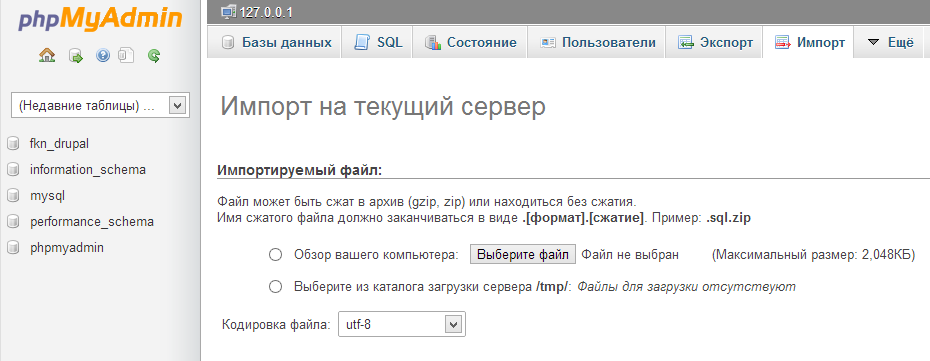
\includegraphics[scale=0.65]{img/import.png}}
\caption{Веб-приложение phpMyAdmin}
\label{pic_phpmyadmin_import}
\end{figure}

При возникновении ошибок подключения срабатывает механизм исключений \lstinline{PDOException}. Для того, чтобы отловить исключение, поместите операции с PDO в блок \lstinline{try ... catch}. С помощью метода \lstinline{getMessage()} можно получить сообщение об ошибке, вызвавшей исключение. Пример такого подключения приведен в листинге~\ref{php_mysql_connect_ex}.  Чтобы закрыть соединение, нужно уничтожить объект, это можно сделать путем присвоения переменной, которая содержит объект, значения \lstinline{null}. Уничтожение объекта обязательно в том случае, когда после получения данных предполагается достаточно большая их обработка.  

%----!!!Обратите внимание на шапку листинга!!!
\begin{lstlisting}[language=PHP, caption={Установка соединения с базой данных}, label=php_mysql_connect_ex]
$user = 'root';
$pswd = '';
try {
	$db = new PDO('mysql:host=localhost;dbname=world', $user, $pswd);
	foreach($db->query('SELECT * FROM cities') as $row)
		print_r($row);
	$db = null;
} catch (PDOException $e) {
	print "Error!: " . $e->getMessage() . "<br/>";
	die(); //Процесс нужно останавливать
}
\end{lstlisting} 

Далее расположен пример программного кода на языке программирования платформы <<1С:Предприятие>>
\begin{lstlisting}[caption={Подключение механизма сканирования}, label=scaner]
&НаКлиенте
Процедура Сканировать(Команда)
 #Если МобильноеПриложениеКлиент Тогда
  Если СредстваМультимедиа.ПоддерживаетсяСканированиеШтрихКодов() Тогда
   ОбработчикСканирования = Новый ОписаниеОповещения(
    "ОбработкаОтсканированногоШтрихкода", ЭтаФорма);
   СредстваМультимедиа.ПоказатьСканированиеШтрихКодов(
    "Сканируйте Штрихкод", ОбработчикСканирования,,
     ТипШтрихКода.Линейный);
  Иначе
   Сообщить("Сканирование штрихкодов не поддерживается!");
  КонецЕсли;
 #КонецЕсли
КонецПроцедуры
\end{lstlisting}


%-------------
%Заключение 
%-------------
\mynonumbersection{Заключение}

В результате выполнения дипломной работы были получены следующие результаты:

\begin{itemize}
\item результат 1; 
\item результат 2;
\item результат 3;
\item результат 4.  
\end{itemize}


    
%-------------
%Список литературы
%-------------
\newpage
%Для включения в диплом списка литературы подключается файл literature.bib
%В нем приведены наиболее часто встречающиеся типы библиографических ссылок
\renewcommand{\refname}{СПИСОК ИСПОЛЬЗОВАННЫХ ИСТОЧНИКОВ}
\addcontentsline{toc}{section}{\refname}
\printbibliography

%-------------
%Приложения
%-------------
\addappendix{UML-диаграмма классов основного модуля приложения}
\label{app-diagram}

В приложении можно разместить основные элементы исходного текста программы или большие рисунки.  

\addappendix{Результаты работы программы}
\label{app-results}

В приложении можно разместить основные элементы исходного текста программы или большие рисунки.  

\end{document}

